\documentclass[11pt,a4paper]{article}
\usepackage{fontspec}
\setmainfont{TeX Gyre Pagella}
\newfontfamily\headfont{Inter}[UprightFont=*-ExtraBold,BoldFont=*-ExtraBold,Extension=.otf,Path=/usr/share/fonts/opentype/inter/]
\usepackage[a4paper,margin=2.3cm]{geometry}
\usepackage{graphicx,booktabs,float,caption,array,xcolor,longtable}
\usepackage{xurl}
\usepackage[hidelinks]{hyperref}
\usepackage{titlesec}
\usepackage[round]{natbib}
\usepackage{setspace}
\setstretch{1.05}
\renewcommand{\topfraction}{0.9}
\renewcommand{\bottomfraction}{0.8}
\renewcommand{\textfraction}{0.1}
\renewcommand{\floatpagefraction}{0.75}
\setlength{\parindent}{0pt}
\setlength{\parskip}{0.55em}
\titleformat{\section}{\headfont\Large}{\thesection}{0.8em}{}
\titleformat{\subsection}{\headfont\large}{\thesubsection}{0.8em}{}
\captionsetup{font=small,labelfont=bf}
\urlstyle{same}
\hypersetup{pdftitle={Ptolemy's World, Measured},pdfauthor={Tristan Hotham}}

\begin{document}
\begin{center}
{\Large\bfseries Ptolemy's World, Measured\par}
\vspace{0.4em}
{\large The coordinates of the Geography set against a modern map:\\2,358 identified places, the stretch in longitude, and the regions Ptolemy drew best and worst\par}
\vspace{1.2em}
{\large Tristan Hotham\par}
\vspace{0.3em}
{\small Independent researcher\\
ORCID: 0000-0003-4931-9349\\
DOI: https://doi.org/10.5281/zenodo.23882603\par}
\vspace{0.8em}
2026
\end{center}

\begin{quote}
\small
\begin{center}\textbf{Abstract}\end{center}
Ptolemy's Geography (about AD 150) records the known world as a table of longitudes and latitudes. Using Grasshoff and Defaux's open catalogue of its main books (10,049 entries, 6,372 with coordinates), I matched the editors' modern identifications of 2,439 point features to modern coordinates through the Pleiades gazetteer, the Digital Atlas of the Roman Empire and hand-located coastal landmarks, giving 2,358 distinct places (74\% at high confidence), and compared his coordinates with the real positions. Read as written and aligned on Alexandria, the median place is 425 km out, and the error grows with distance from Alexandria (rank correlation 0.91). Almost all of this is a stretch in longitude: real longitude is best predicted by 0.72 times Ptolemy's, within 0.6\% of the ratio 500/700 implied by his small Earth, and this three-parameter correction reduces the median error to 144 km, as low as a six-parameter affine fit (142 km). Regional distortions remain: Scotland is turned 78 degrees clockwise relative to England, the Indian peninsula spans 3.8 rather than 13.6 degrees of latitude, Taprobane (Sri Lanka) covers about 14.6 times its real area, and the Caspian, correctly enclosed, is as wide as it is long. After each regional map's own best similarity transform, Sardinia and Sicily, Thrace and Greece are drawn best (median 42 to 52 km) and India worst (528 km). The Omega and Xi recensions agree exactly for 69\% of shared entries and fit reality equally well.

\textbf{Keywords:} Ptolemy; Geography; ancient cartography; historical geography; map distortion; Pleiades; open data
\end{quote}

\section{Introduction}
Claudius Ptolemy's \textit{Geography}, compiled in Alexandria around AD 150, is a manual of mapmaking and a table. Its first book discusses the size of the Earth, the sources, and two projections; Books 2 to 7 list some eight thousand localities, province by province, each with a longitude counted in degrees east of the Fortunate Isles and a latitude north or south of the equator; Book 8 divides the world into 26 regional maps. The coordinates shaped the European picture of the world from their rediscovery in Byzantium around 1300 until the sixteenth century.

The distortions of Ptolemy's world are well known in outline: the inhabited world is stretched from east to west, Scotland is turned towards the east, India is truncated while Taprobane is enlarged, and the Indian Ocean is closed by an unknown southern land. This paper measures them on a large set of identified places, using an open edition of the coordinates \citep{cat} and open gazetteers, and reports how much of the error a single simple correction removes. It accompanies an interactive comparison of Ptolemy's coordinates and a modern map (\url{https://maps.tristanhotham.com/ptolemy/}).

\section{Data}
\textbf{The catalogue.} \citet{cat} give, for every entry of Books 2 to 7, an identifier (book, chapter, section, entry), the regional map, the name in German, the editors' modern identification in German (blank where unknown), and longitude and latitude in the Omega and Xi recensions. There are 10,049 entries; 6,372 have coordinates (6,338 in Omega, 4,440 in Xi, 4,406 in both). Ptolemy's longitudes run from 1 to 180 degrees and his latitudes from -15.0 to 63.2.

\textbf{Gazetteers.} Pleiades version 4.1 \citep{pleiades}, with ancient and modern names and place types; the Digital Atlas of the Roman Empire \citep{dare}, with Latin, Greek and modern names; and Natural Earth towns and outlines \citep{naturalearth}.

\section{Methods}
\textbf{Feature types.} Each entry was classed by its German name as a settlement, cape, river mouth, harbour, island, river source, point along a river, mountain, boundary point or lake. Only the point features (settlements, capes, mouths, harbours, islands) were used: 5,667 with coordinates, of which the editors identify 2,871 (51\%). Unidentified entries were never matched.

\textbf{Matching.} An identified entry was matched to a gazetteer place inside a generous box around its chapter's region when (high confidence) the place's ancient names contain Ptolemy's name and its modern names contain the editors' identification (1,436 places), or (medium) one of the two names matches a single place, all candidates lying within 25 km of each other (261 by ancient name, 202 by modern name). Names were compared on skeletons that ignore Greek and Latin orthography and German transliteration; Pleiades places typed as regions, rivers, peoples or mountains could not match a settlement. Capes, river mouths, estuaries and some cities beyond the gazetteers were located by hand for the editors' identification (459 places, each marked high or medium). Ptolemy's errors are spatially smooth, so each match was compared with its eight nearest neighbours on his map: the residual of a simple per-region fit was compared with the neighbours' median. 21 medium matches departing by more than 300 km were dropped; high and hand matches departing that much were inspected one by one and 2 rejected. Where one real place appears twice the first entry was kept. The result is 2,358 places with Omega coordinates: 1,365 in Europe, 297 in Africa and 696 in Asia.

\textbf{Transforms.} Errors are great-circle distances between the real place and the position a transform assigns to Ptolemy's coordinates. F0 shifts his longitudes so that Alexandria falls in place and keeps his latitudes. F1 fits modern longitude as $a + b\lambda_P$ and modern latitude as $\varphi_P + c$ by least squares (longitude residuals weighted by the cosine of latitude). F2 is a general affine transform; F3 a Helmert (similarity) transform between grids drawn with the aspect of the parallel of Rhodes, 36 degrees; F4 is F1 fitted per regional map. The shape error of a region is the residual of a Helmert transform fitted to that region alone in local kilometres.

\begin{table}[tbp]\centering\small\caption{Error of each transform from Ptolemy's coordinates to modern ones (km).}\label{tab:fits}\begin{tabular}{lrrrr}\toprule Transform & Parameters & Median & RMS & 90th pct.\\\midrule
F0 as written (aligned on Alexandria) & 0 & 425 & 751 & 1,340\\
F1 longitude stretch and shift & 3 & 144 & 286 & 435\\
F2 affine & 6 & 142 & 240 & 331\\
F3 Helmert (rotation, scale, shift) & 4 & 144 & 257 & 371\\
F4 F1 per regional map & 3 per map & 105 & 181 & 241\\
\bottomrule\end{tabular}\end{table}

\section{Results}
\subsection{The stretch in longitude}
From Cape St Vincent to Sera (taken by the editors as Xi'an), Ptolemy counts 174.8 degrees of longitude against a real 117.9, a stretch of 1.48. Measured from Alexandria, Ptolemy's longitude difference is 1.37 times the real one (Figure~\ref{fig:stretch}), on both sides of Alexandria. The fitted F1 factor is $b = 0.7189$ (Europe 0.691, Africa 0.716, Asia 0.729). Ptolemy adopted a degree of 500 stadia where Eratosthenes had 700; if distances in stadia were broadly right, his degrees should be shrunk by $500/700 = 0.714$, which $b$ matches to within 0.6\%. On F1 his prime meridian falls at 12.9 degrees west.

\begin{figure}[tbp]\centering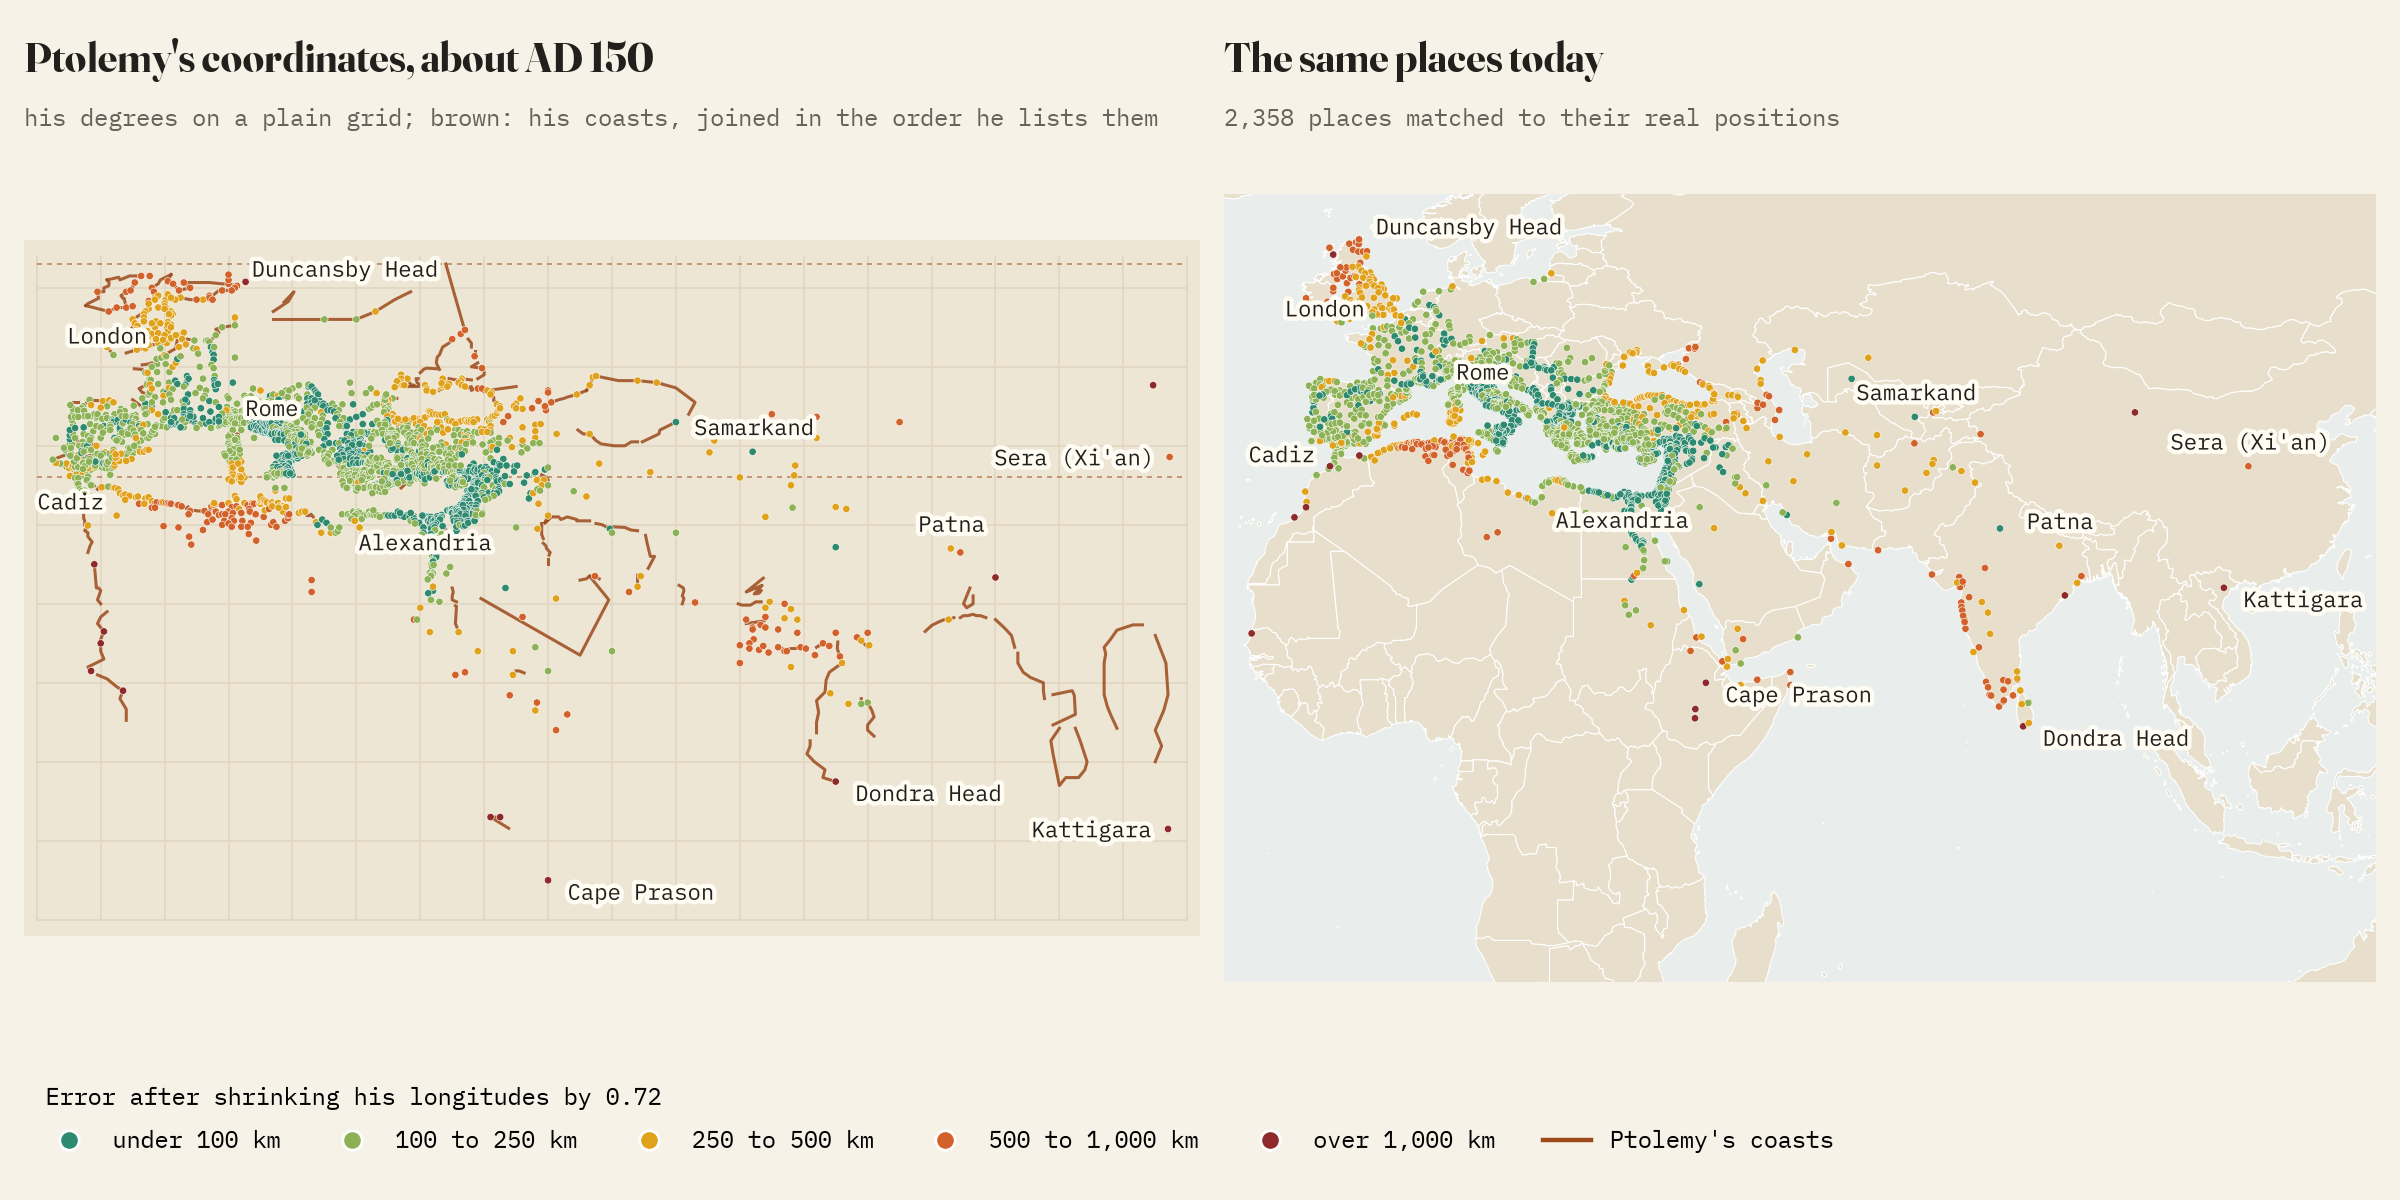
\includegraphics[width=\textwidth]{f_maps.png}
\caption{Ptolemy's coordinates on a plain grid of his degrees (left; his coasts joined in the order he lists them) and the matched places at their real positions (right), coloured by error under F1.}\label{fig:maps}\end{figure}

\begin{figure}[tbp]\centering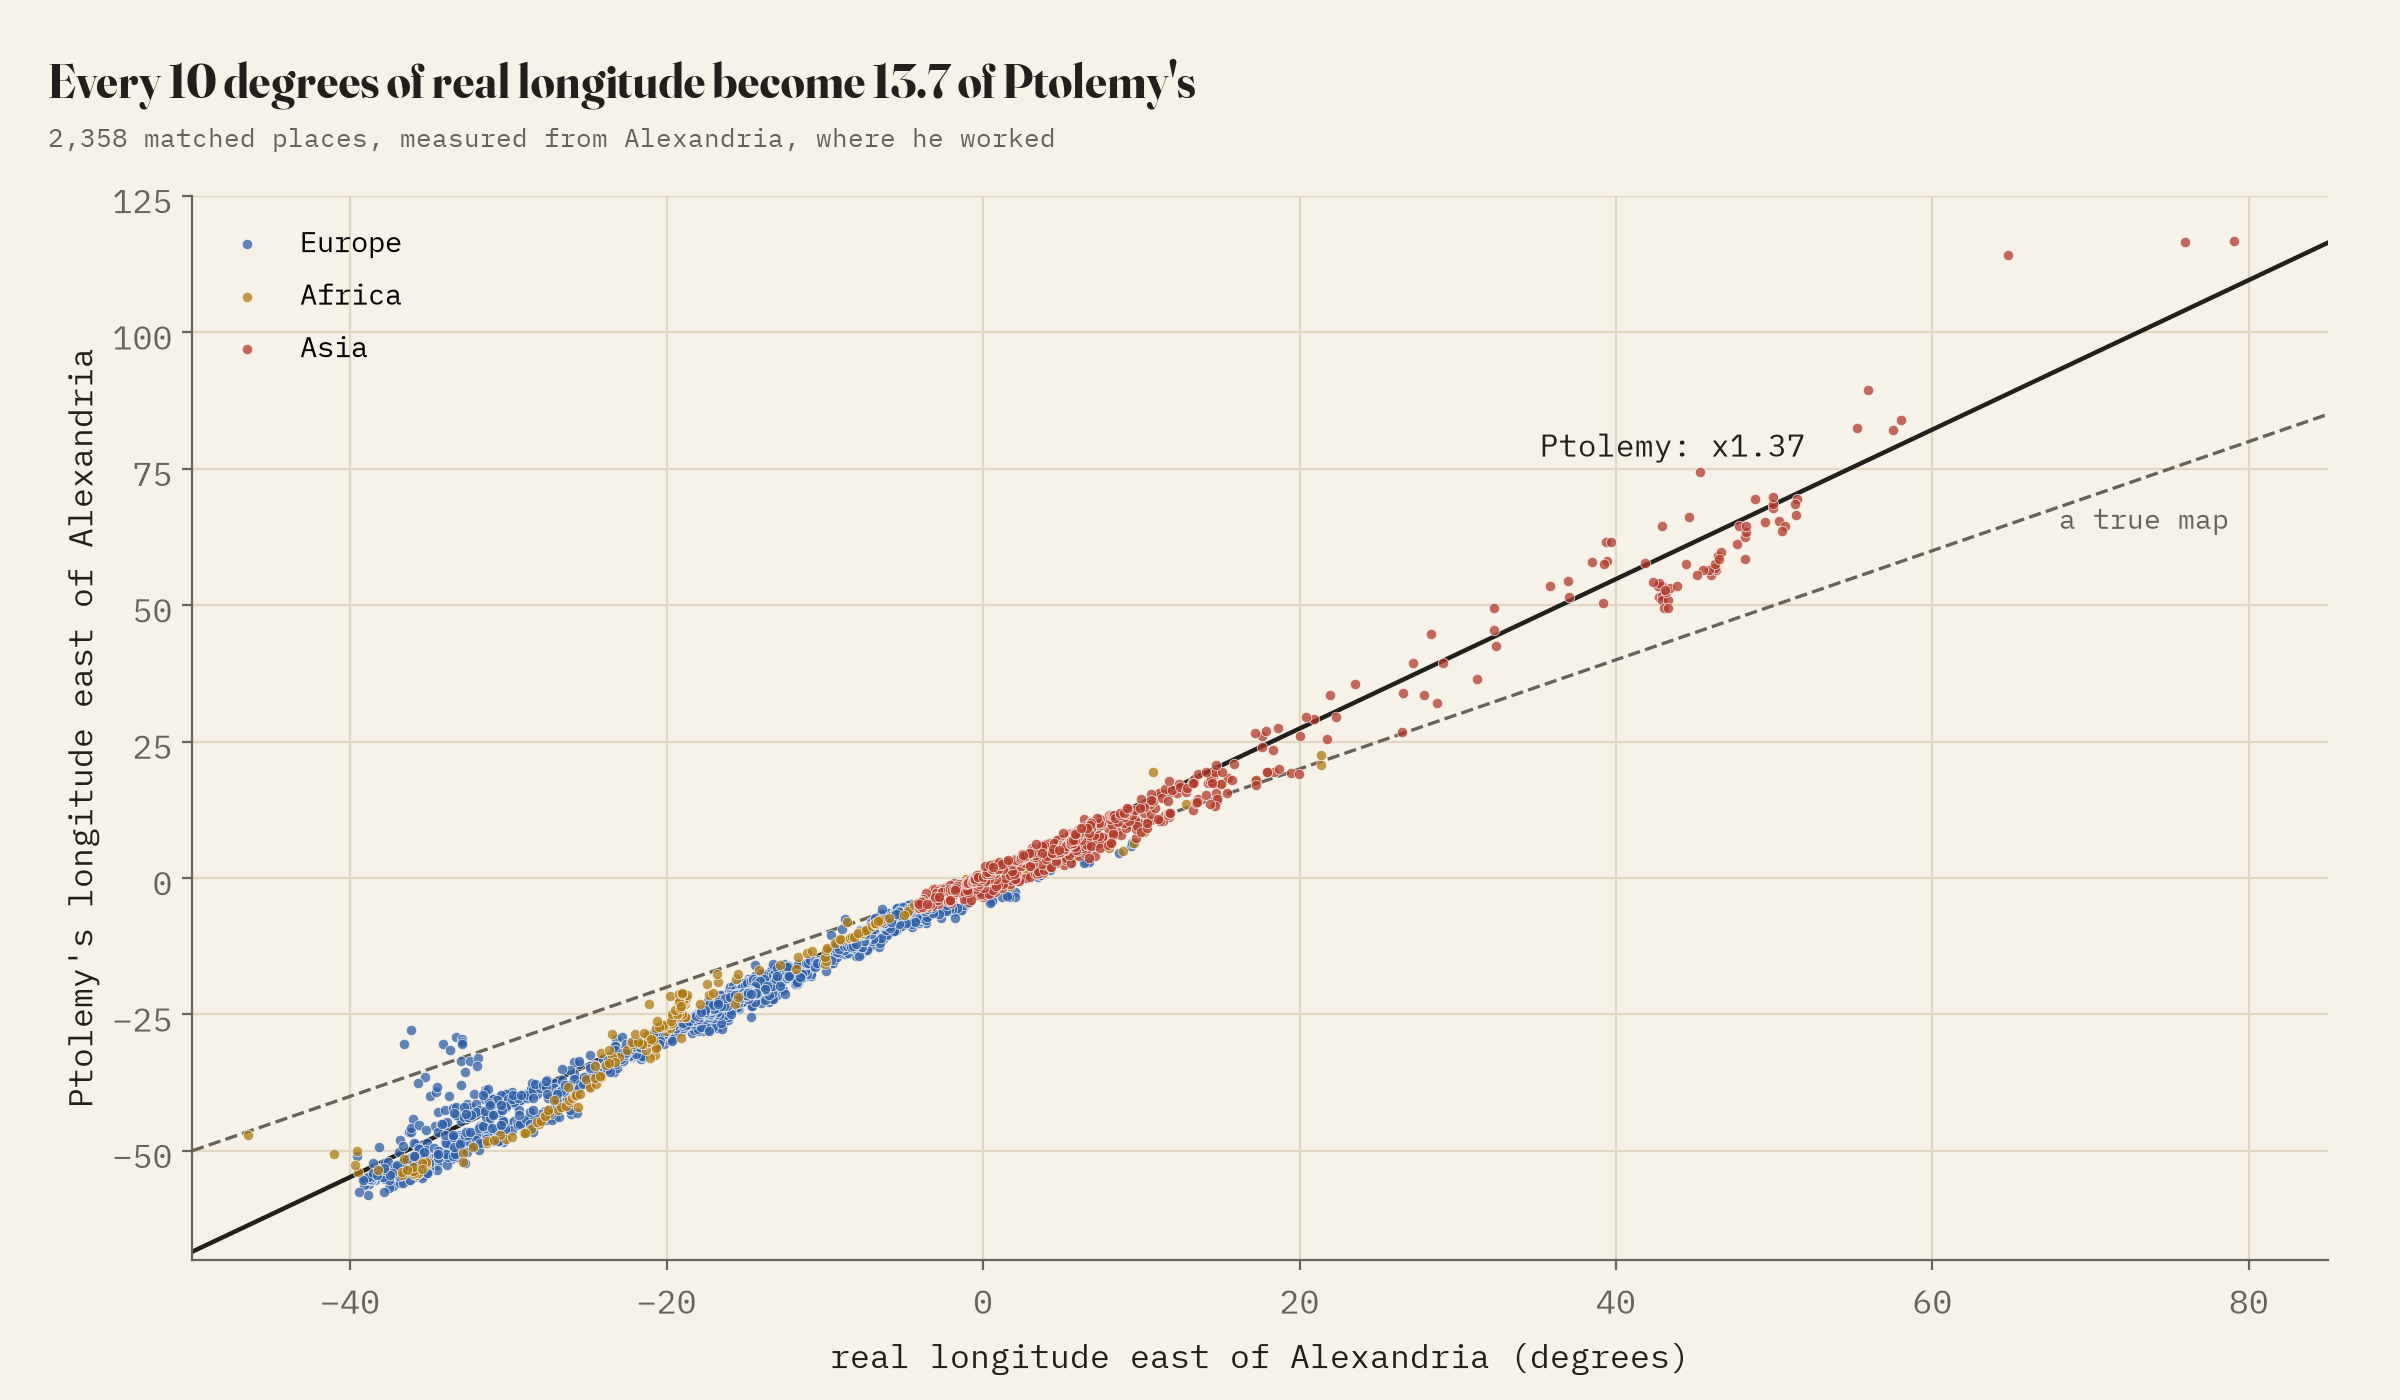
\includegraphics[width=\textwidth]{f_stretch.png}
\caption{Ptolemy's longitude difference from Alexandria against the real one.}\label{fig:stretch}\end{figure}

\subsection{Error and distance from Alexandria}
Under F0 the median error rises from 134 km within 1,000 km of Alexandria to 1,445 km beyond 4,000 km (56 places); the rank correlation of error with distance from Alexandria is 0.91, falling to 0.44 under F1 (Figure~\ref{fig:alex}). The median F0 error is 28\% of the distance from Alexandria. Latitudes are better than longitudes: the median absolute latitude error is 0.77 degrees and 58\% are within a degree, but they are biased regionally, by 3.0 degrees in the British Isles and -4.1 in Roman Africa.

\begin{figure}[tbp]\centering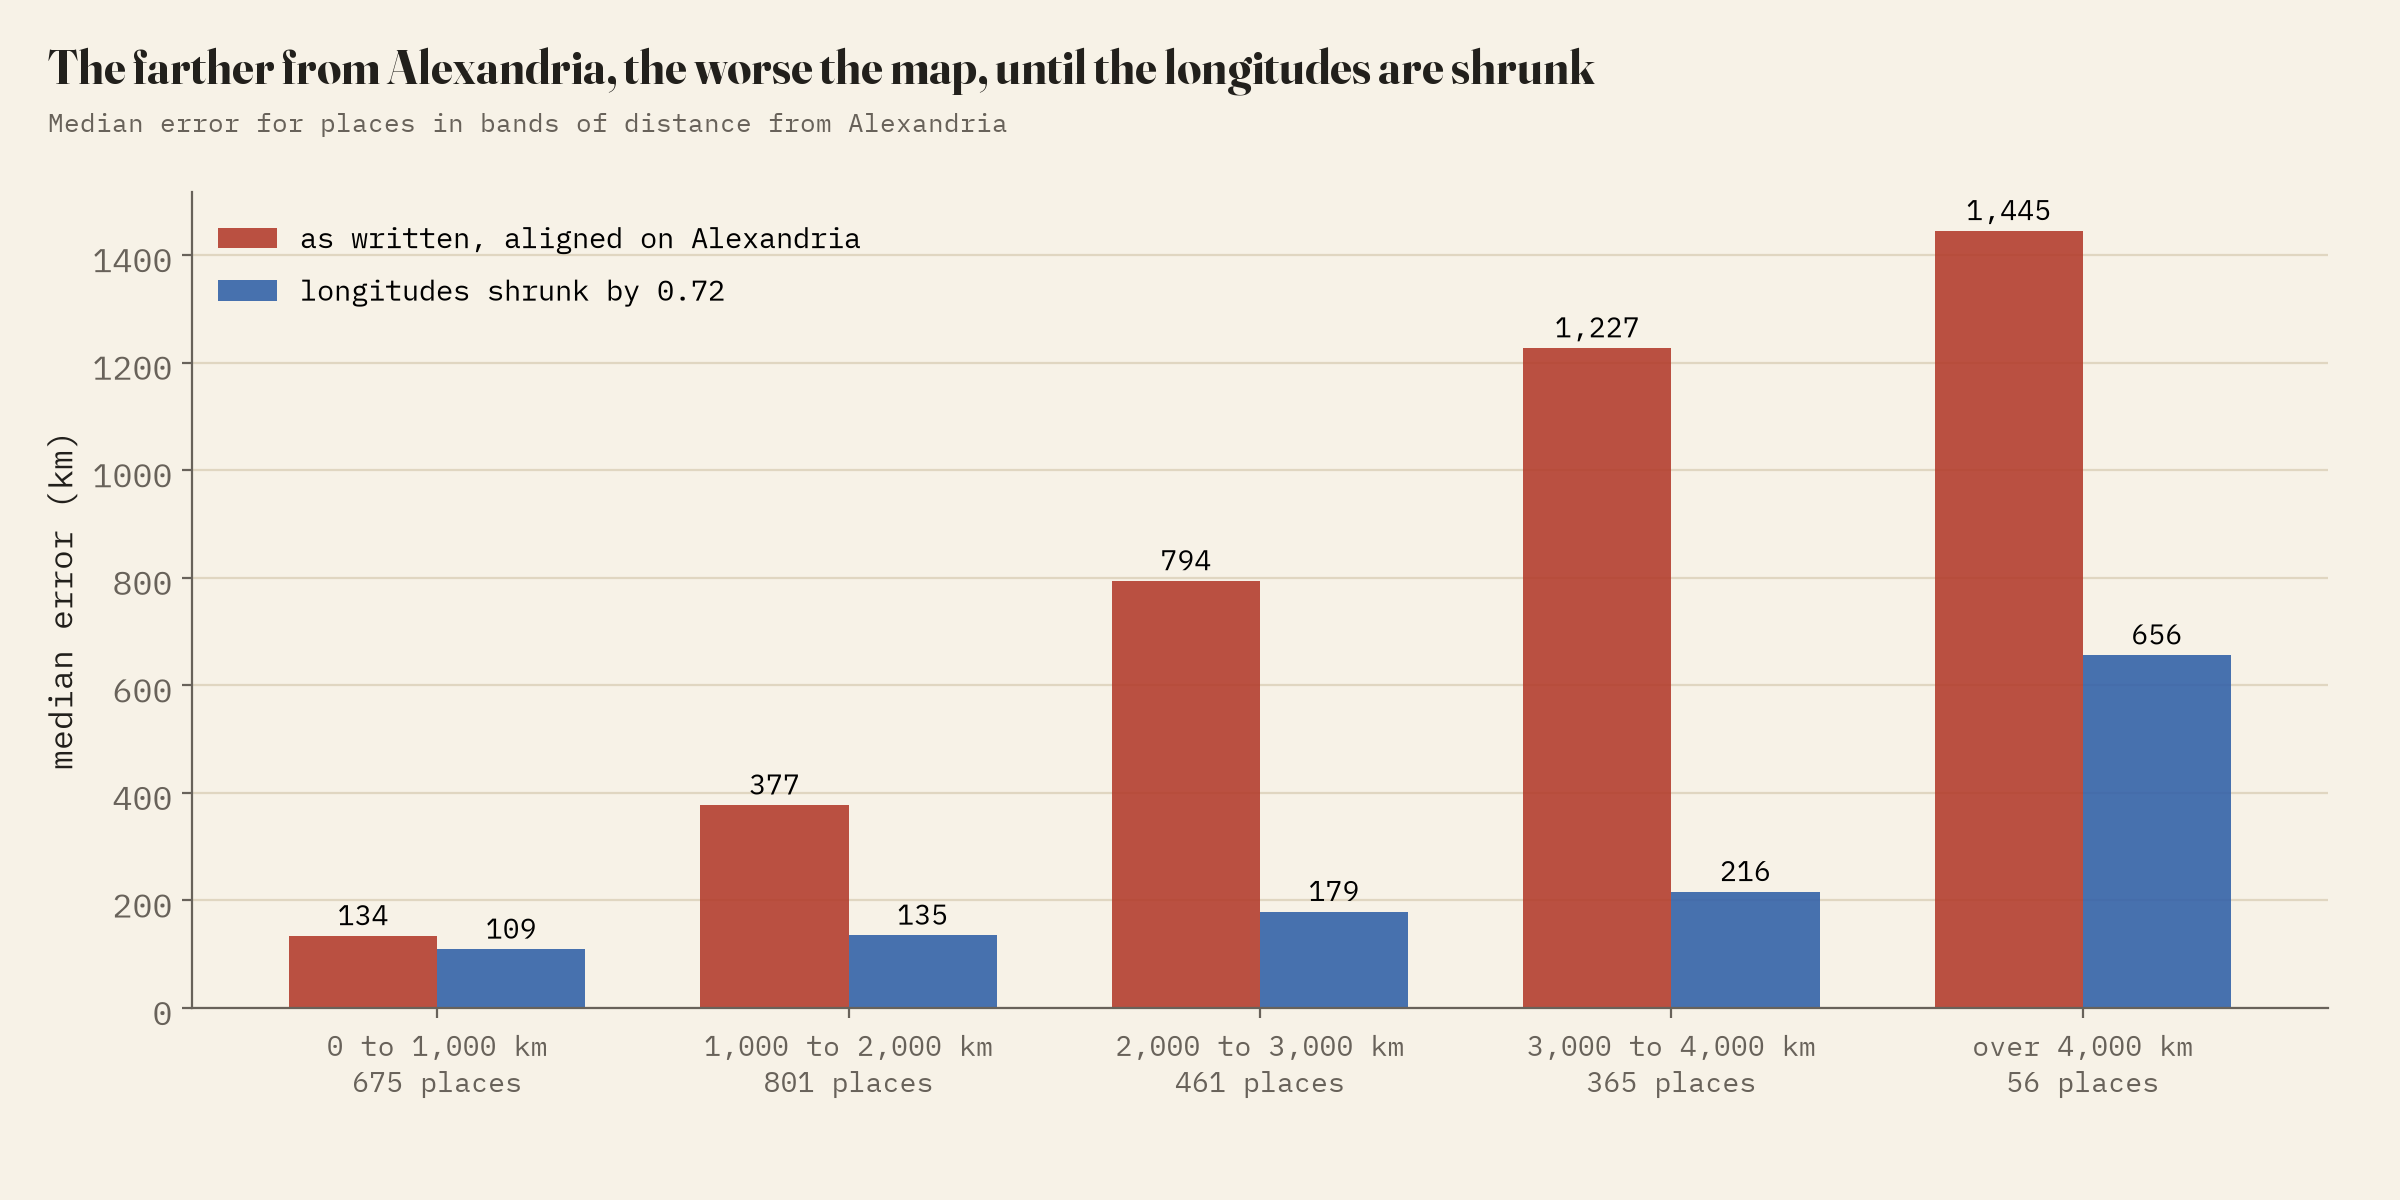
\includegraphics[width=\textwidth]{f_alex.png}
\caption{Median error by distance from Alexandria, as written and under F1.}\label{fig:alex}\end{figure}

\begin{figure}[tbp]\centering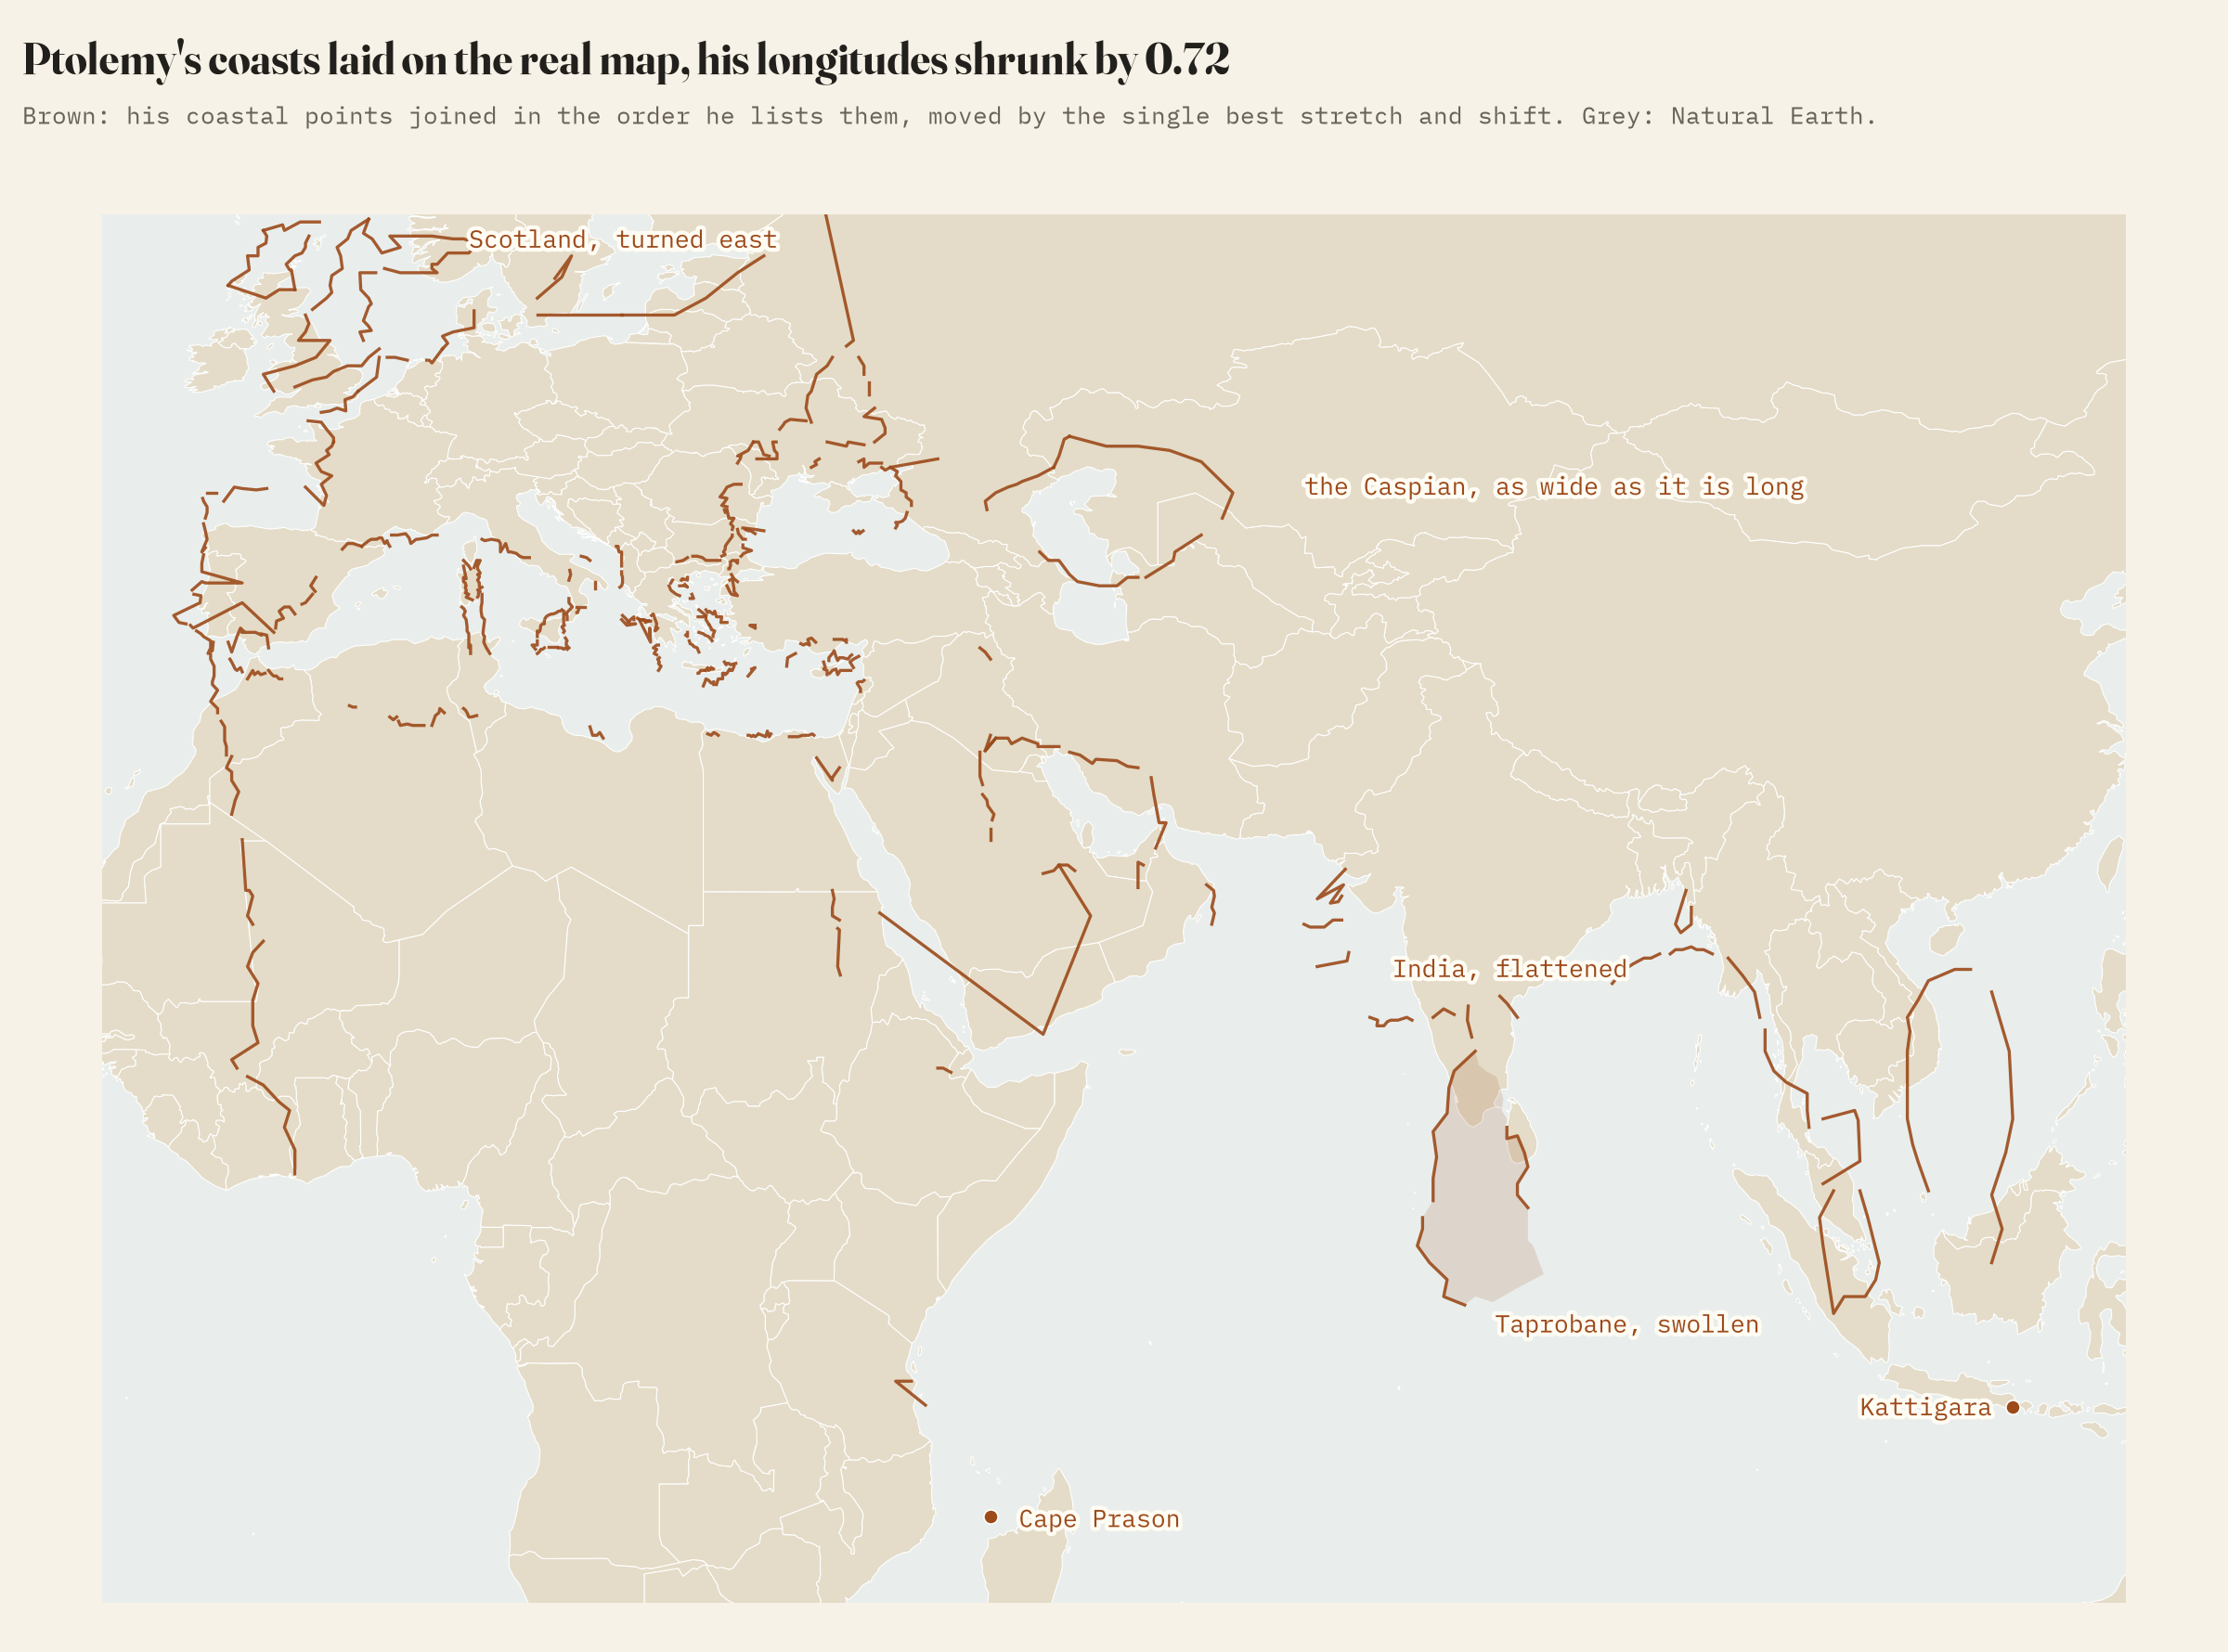
\includegraphics[width=\textwidth]{f_overlay.png}
\caption{Ptolemy's coasts transformed by F1 and laid on the real map.}\label{fig:overlay}\end{figure}

\subsection{Scotland, India, Taprobane}
Fitted separately, Ptolemy's Scotland (22 places north of 55 degrees) is rotated 87.1 degrees and his England and Wales (60 places) 8.9 degrees, a relative turn of 78.2 degrees clockwise; the bearing from the Solway Firth to Duncansby Head is 3 degrees in reality and 79 on his map (Figure~\ref{fig:britain}).

From Barygaza (Bharuch) to Cape Komaria (Cape Comorin) is 13.6 degrees of latitude in reality and 3.8 on Ptolemy's map; Komaria is 5.4 degrees too far north and the coast between runs at 115 instead of 161 degrees. His Taprobane, the coast in sections 7.4.2 to 7.4.7 (36 points), spans 15.0 degrees of latitude, from 12.5 N to -2.5, against 3.9 for Sri Lanka, and encloses 960,744 km$^2$ when his longitudes are scaled by $b$, about 14.6 times the real island's 65,928 km$^2$ (Figure~\ref{fig:india}). Only 6 places in Taprobane and 43 in India are matched, so these figures rest on few points.

\begin{figure}[tbp]\centering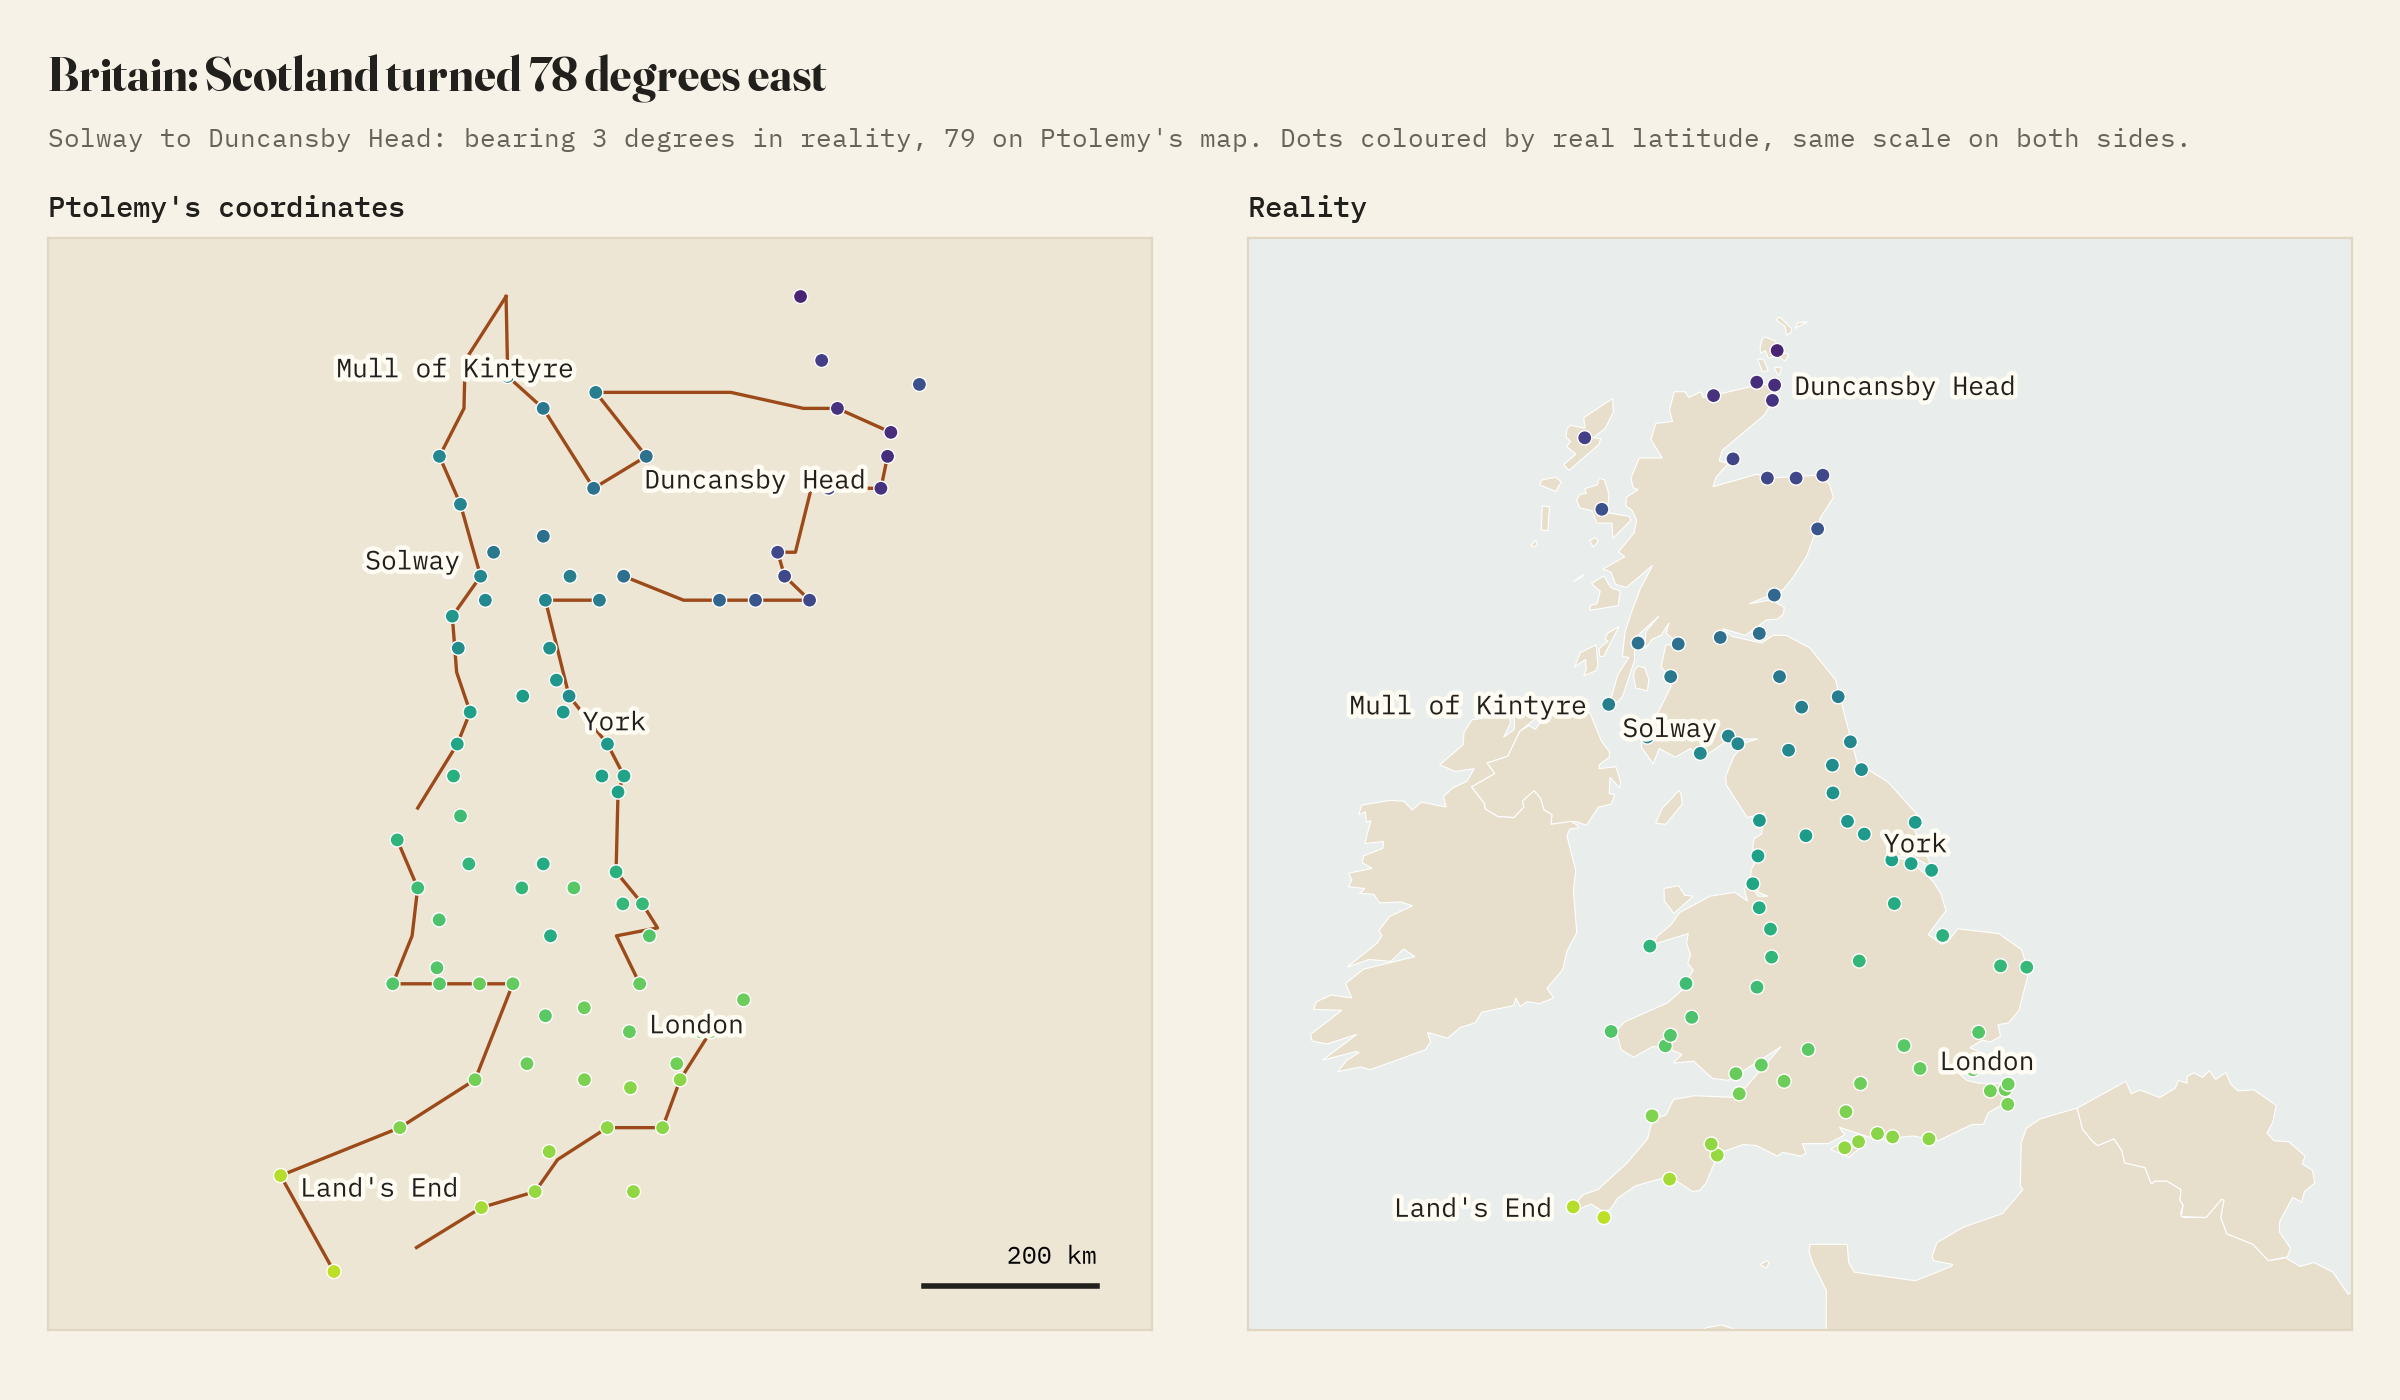
\includegraphics[width=\textwidth]{f_britain.png}
\caption{Britain in Ptolemy's coordinates and in reality, at the same scale.}\label{fig:britain}\end{figure}

\begin{figure}[tbp]\centering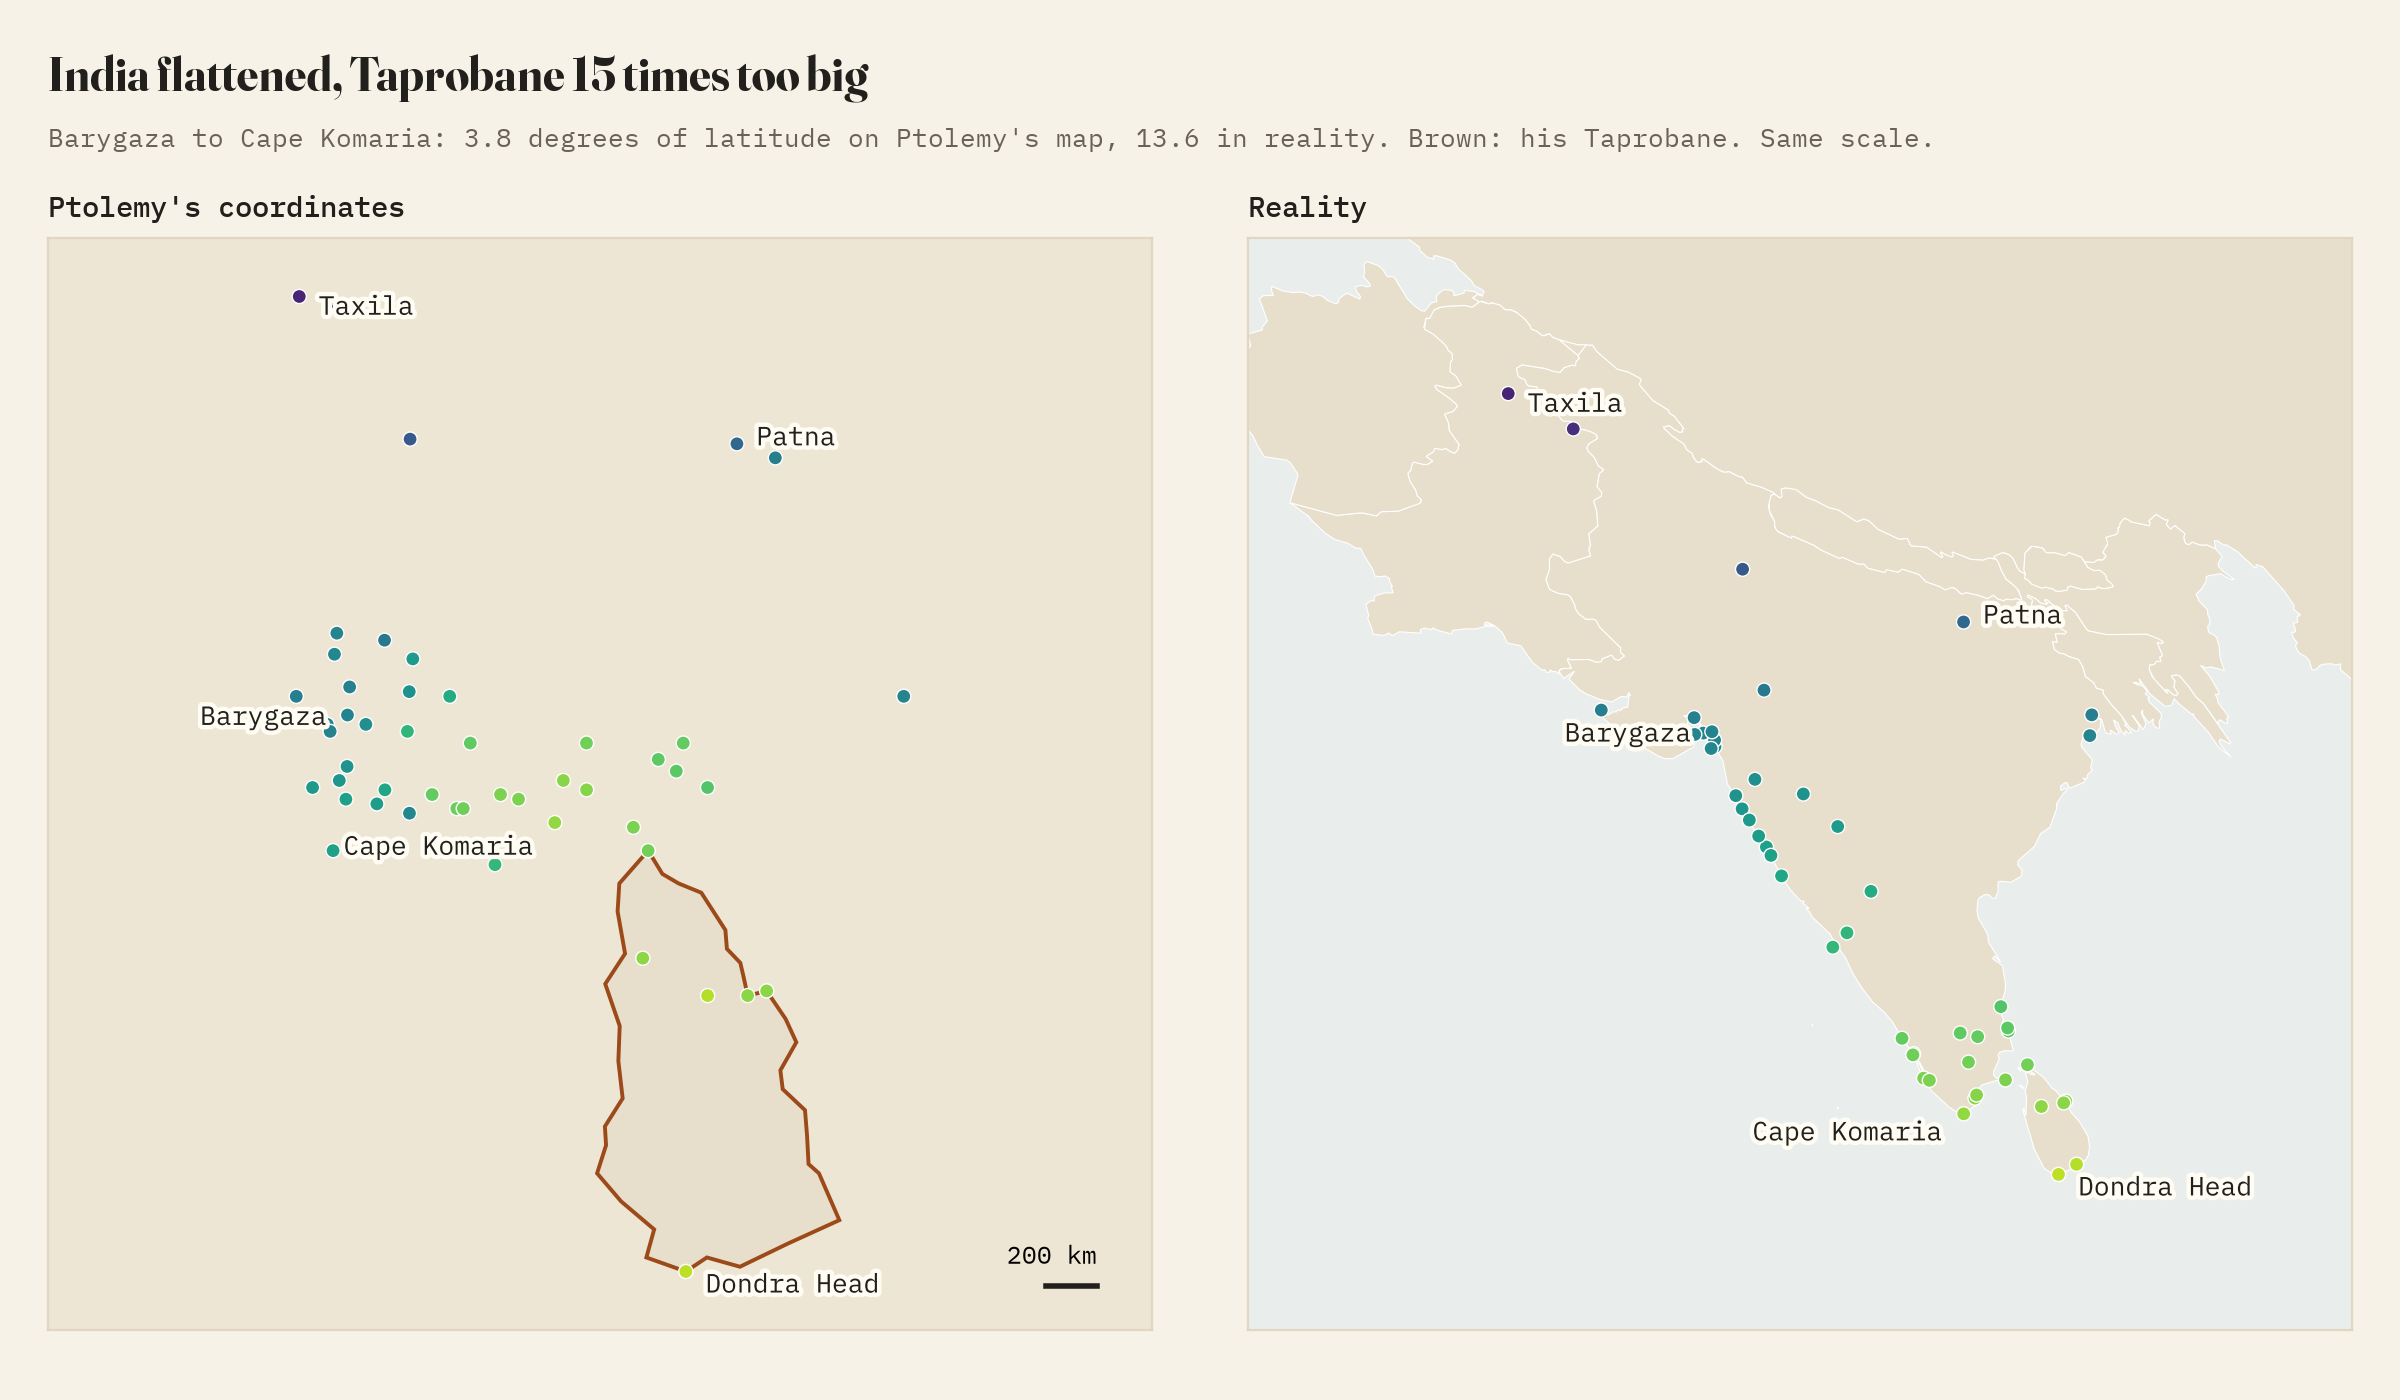
\includegraphics[width=\textwidth]{f_india.png}
\caption{India and Taprobane in Ptolemy's coordinates and in reality, at the same scale.}\label{fig:india}\end{figure}

\subsection{Enclosed seas}
For 8 river mouths on the real Caspian shore, the real spread is 1,054 km north to south and 387 km east to west; Ptolemy's is 815 and 790 km (longitudes scaled by $b$). He brings the Oxus and Jaxartes into the Caspian, though their mouths lie in the Aral Sea 470 and 620 km from its shore (Figure~\ref{fig:caspian}). In the Indian Ocean, Cape Prason (Cape Delgado in the editors' reading) is placed at -15 degrees, 25.7 degrees too far south, and Kattigara (near Hanoi in their reading) at -8.5, 29.5 degrees too far south and 3,403 km from its F1 position; the text joins the two by unknown land.

\begin{figure}[tbp]\centering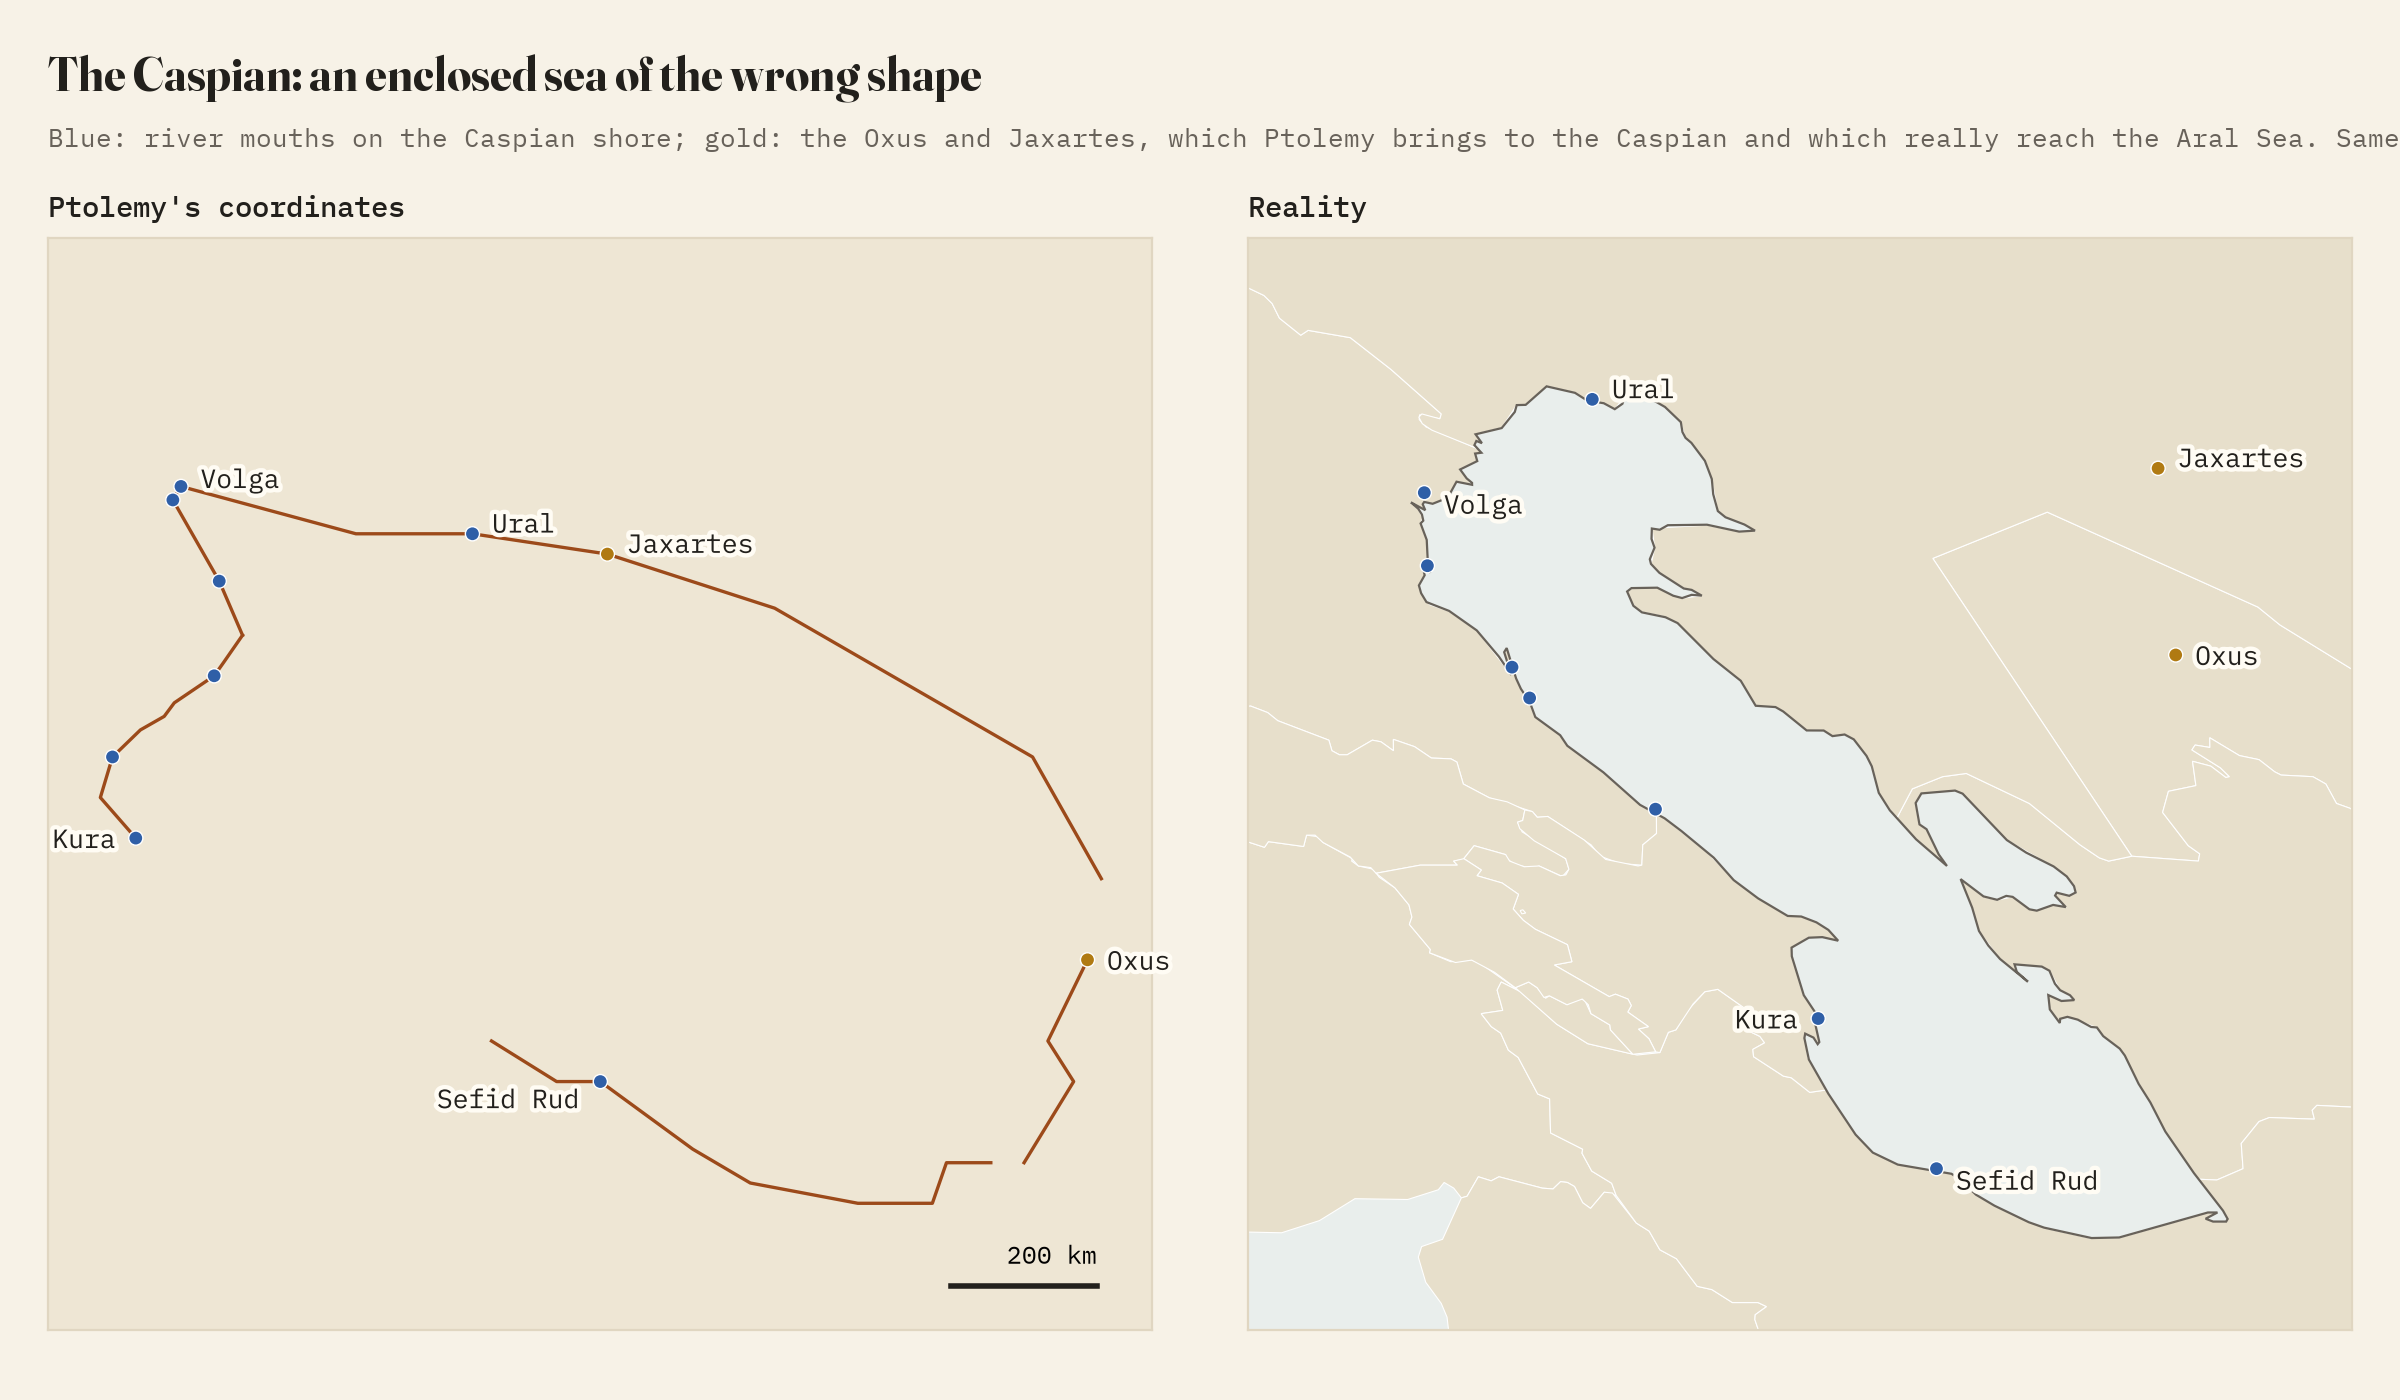
\includegraphics[width=\textwidth]{f_caspian.png}
\caption{The Caspian and the mouths of the Oxus and Jaxartes in Ptolemy's coordinates and in reality.}\label{fig:caspian}\end{figure}

\subsection{Regional maps}
Table~\ref{tab:regions} and Figure~\ref{fig:regions} give the median shape and placement errors for each regional map. Among the 18 maps with at least 15 places, shape error is lowest for Sardinia and Sicily (42 km), Dacia, Moesia and Thrace (52 km) and Greece (52 km), and highest for the British Isles (128 km), Inner Libya and Ethiopia (448 km) and India (528 km). Placement under F1 is best for Cyprus, Syria and Mesopotamia (71 km) and Cyrenaica and Egypt (93 km).

\begin{table}[tbp]\centering\small\caption{Ptolemy's 26 regional maps: matched places, median shape error, median error under F1 and as written (km), and median latitude error (degrees, positive too far north). Shape errors in brackets rest on fewer than 15 places.}\label{tab:regions}\begin{tabular}{lrrrrr}\toprule Regional map & Places & Shape & F1 & F0 & Latitude\\\midrule
British Isles & 92 & 128 & 432 & 746 & +3.0\\
Iberia & 240 & 70 & 187 & 1,382 & +0.5\\
Gaul & 130 & 78 & 126 & 890 & +0.1\\
Germany & 9 & (28) & 183 & 591 & +1.1\\
Alps and Danube & 104 & 85 & 113 & 453 & -0.3\\
Italy and Corsica & 295 & 74 & 101 & 575 & -0.4\\
Sardinia and Sicily & 103 & 42 & 119 & 627 & -0.8\\
Sarmatia and Crimea & 19 & 92 & 375 & 381 & +2.4\\
Dacia, Moesia, Thrace & 83 & 52 & 151 & 353 & +1.1\\
Greece & 290 & 52 & 131 & 270 & -0.7\\
Mauretania & 56 & 96 & 454 & 1,522 & -3.1\\
Roman Africa & 88 & 116 & 491 & 724 & -4.1\\
Cyrenaica and Egypt & 124 & 84 & 93 & 94 & -0.2\\
Inner Libya and Ethiopia & 29 & 448 & 569 & 515 & -4.1\\
Asia Minor & 357 & 84 & 135 & 156 & +0.8\\
Asiatic Sarmatia & 16 & 98 & 441 & 434 & +3.5\\
Caucasus and Armenia & 38 & 108 & 366 & 402 & +2.7\\
Cyprus, Syria, Mesopotamia & 191 & 70 & 71 & 188 & -0.2\\
Media and Persia & 12 & (116) & 234 & 538 & +1.1\\
Arabia & 13 & (264) & 418 & 496 & -1.3\\
Central Asia & 10 & (259) & 406 & 1,338 & +1.6\\
Scythia and Serica & 2 &  & 1,179 & 3,680 & +5.9\\
Afghanistan and Gedrosia & 6 &  & 360 & 1,673 & +1.1\\
India & 43 & 528 & 599 & 1,266 & -0.5\\
Further India and China & 2 &  & 2,202 & 4,496 & -13.2\\
Taprobane & 6 &  & 382 & 1,740 & -0.4\\
\bottomrule\end{tabular}\end{table}

\begin{figure}[tbp]\centering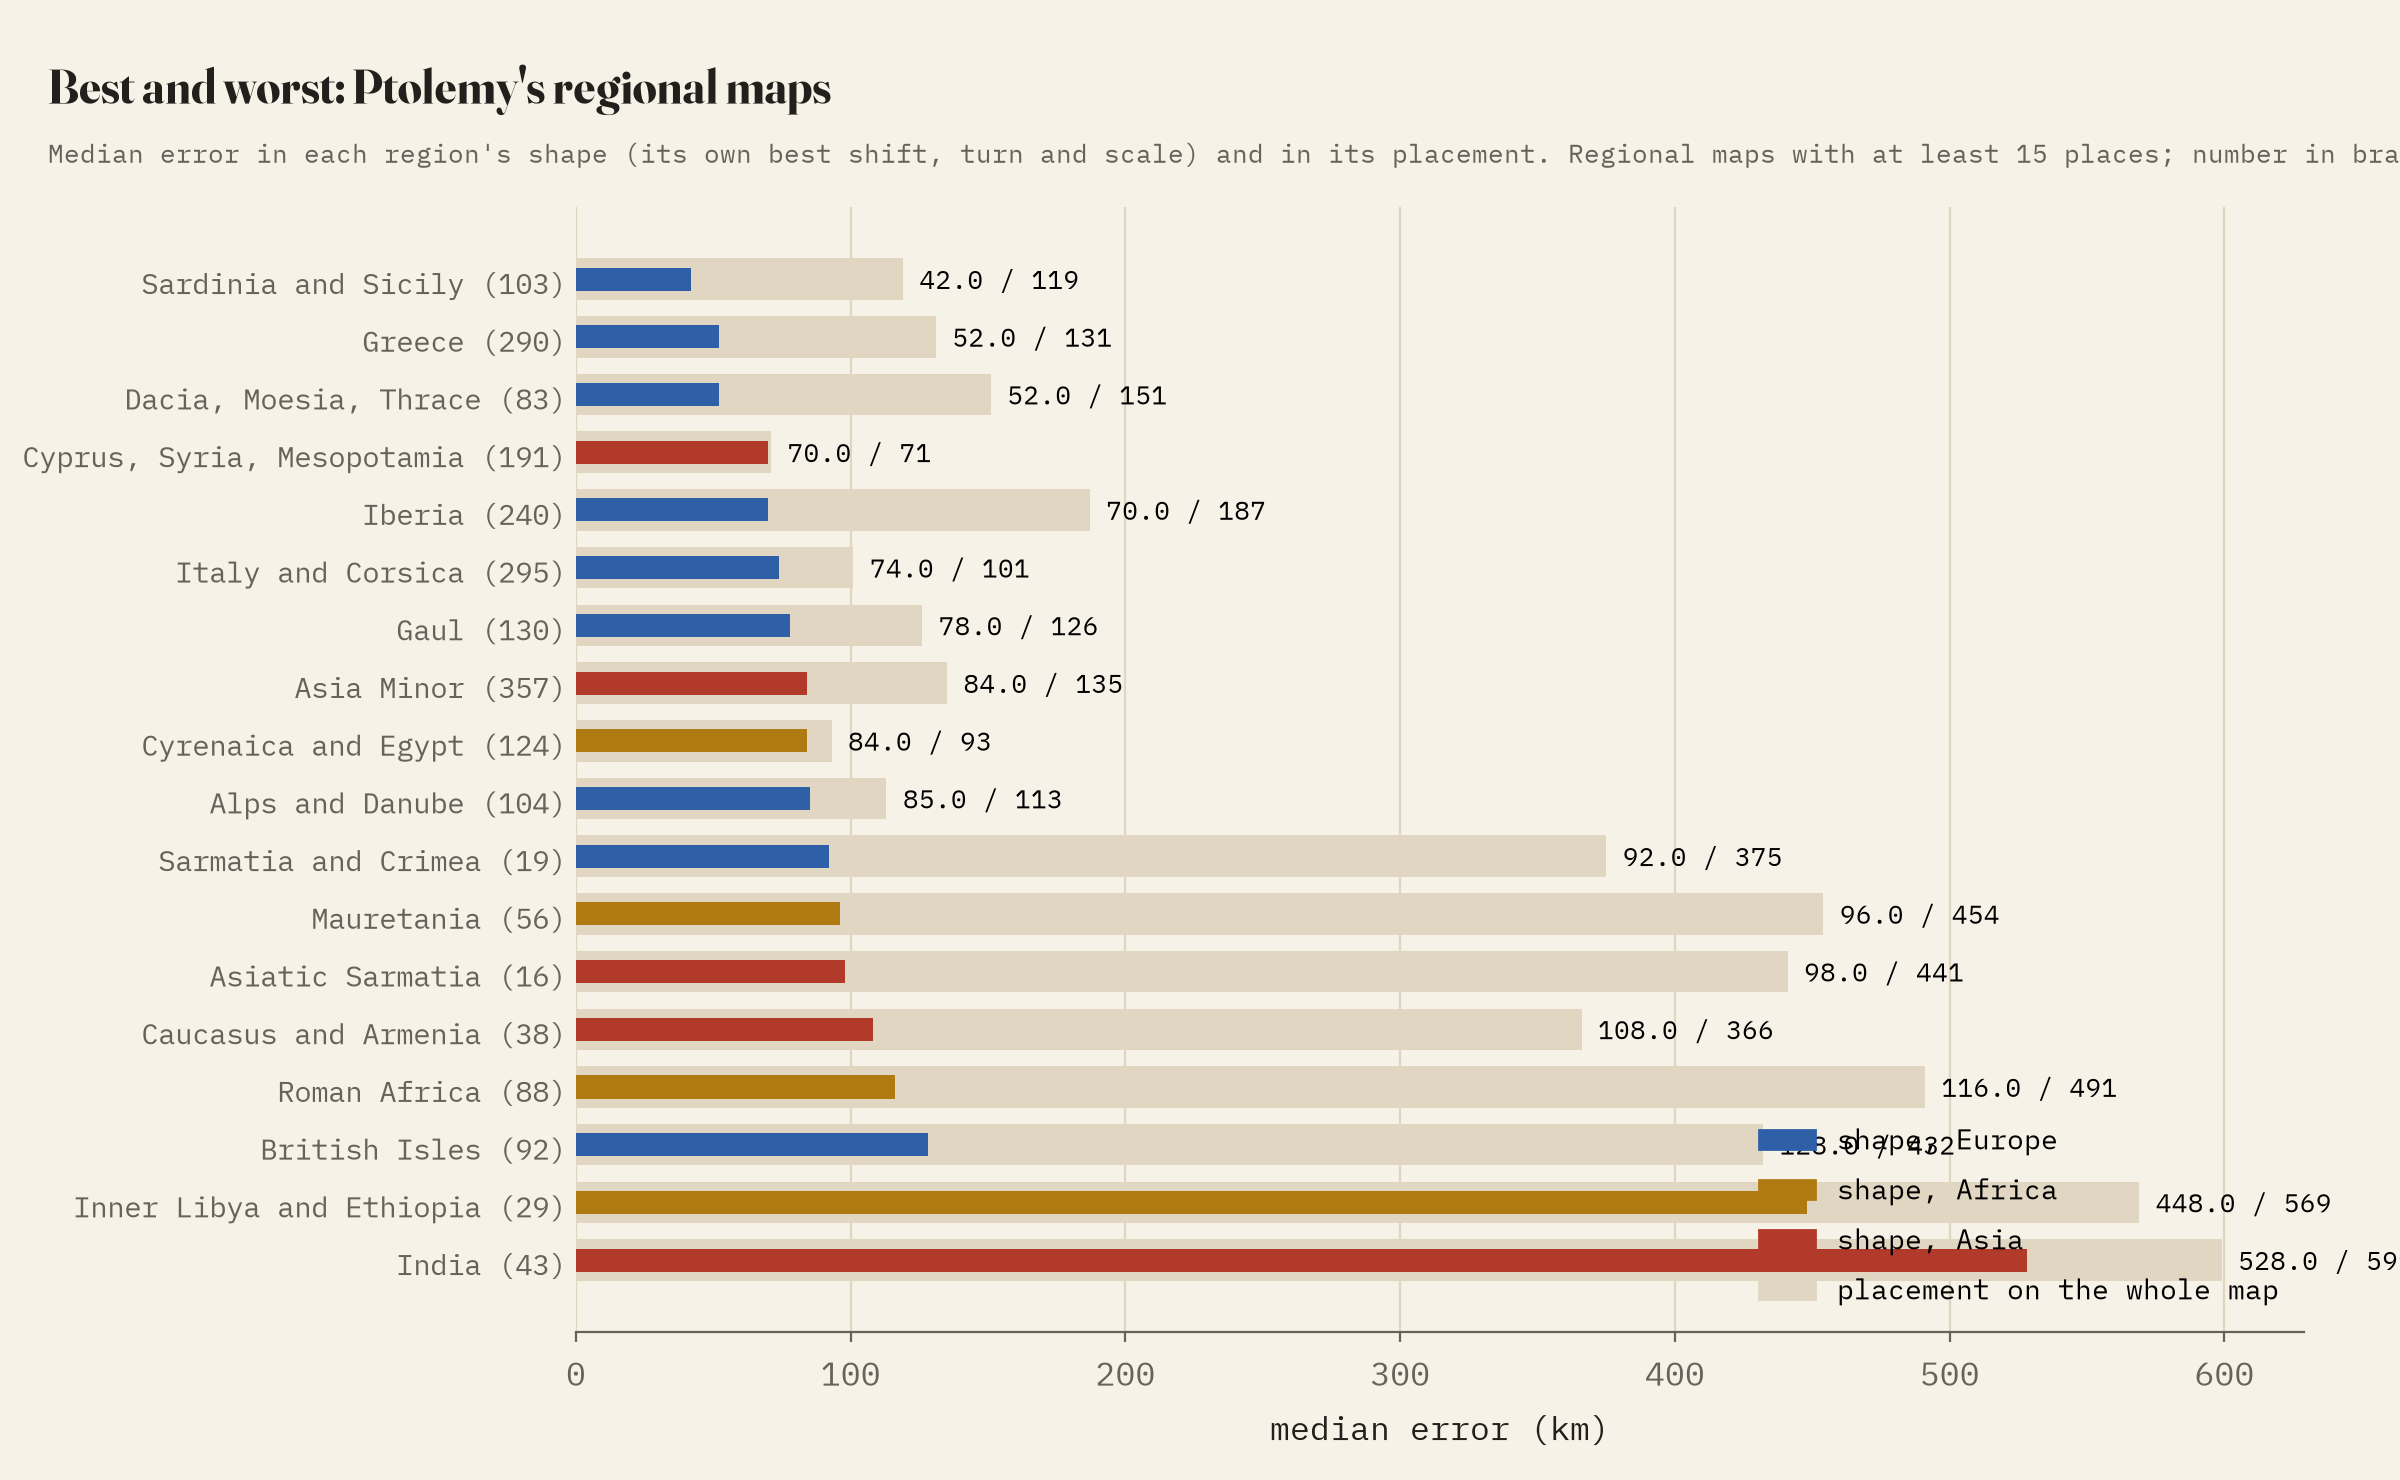
\includegraphics[width=\textwidth]{f_regions.png}
\caption{Median shape and placement error by regional map.}\label{fig:regions}\end{figure}

\subsection{The Omega and Xi recensions}
Of 4,406 entries with coordinates in both recensions, 3,033 (68.8\%) agree exactly; 681 differ only in latitude and 448 only in longitude; the median difference is 20 minutes and 245 differ by a degree or more (Figure~\ref{fig:rec}). Disagreement is highest in Book 2 (41.5\%) and lowest in Book 5 (21.4\%). Fitted by F1 on the 2,049 matched places with both, the two have the same median error (144 km) and stretch (0.711 and 0.7114); where they differ, Xi is closer 364 times and Omega 266 times.

\begin{figure}[tbp]\centering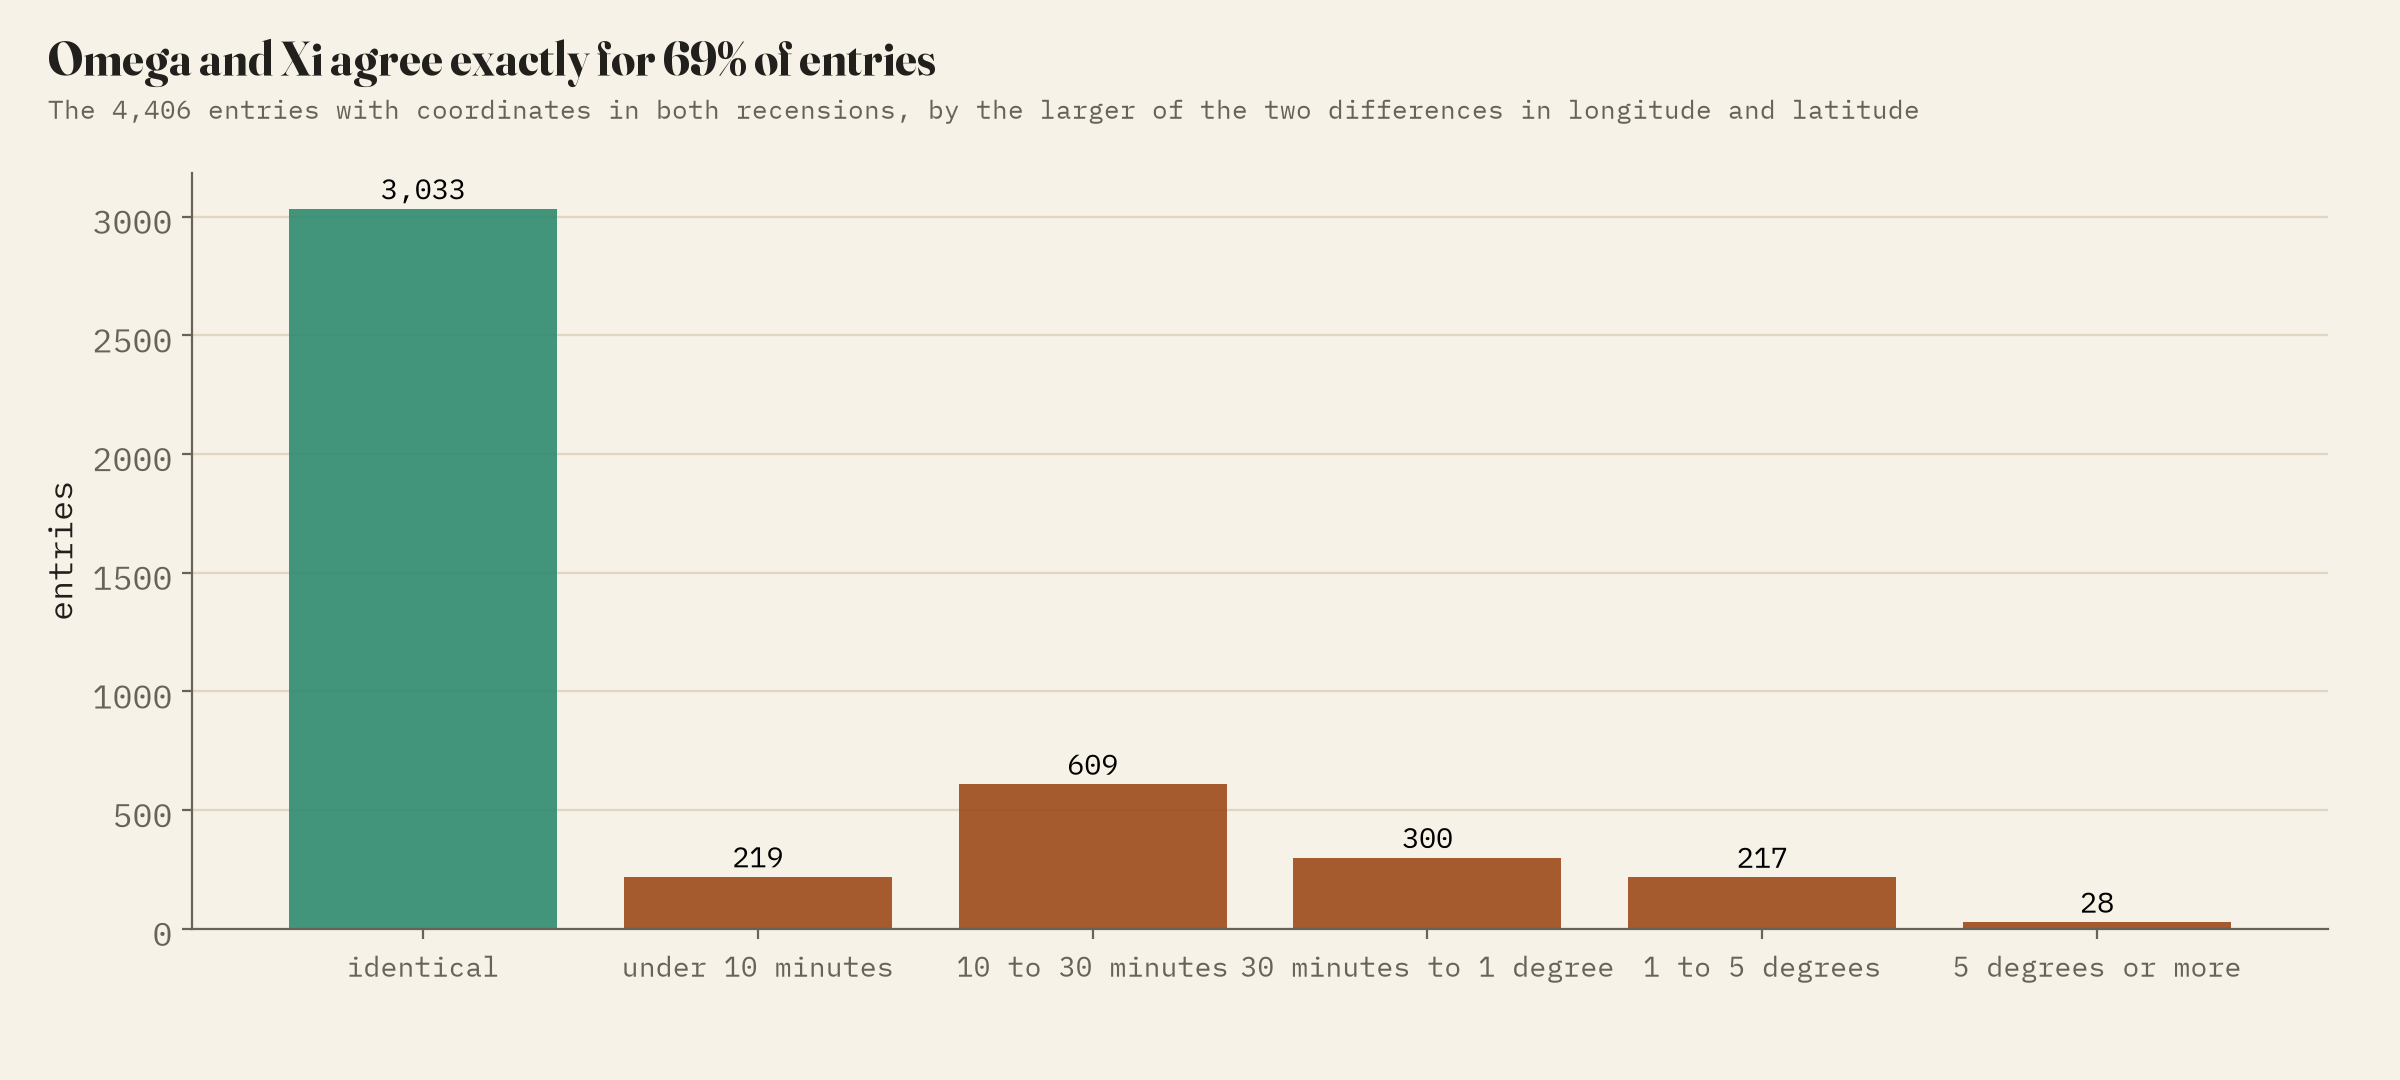
\includegraphics[width=\textwidth]{f_recensions.png}
\caption{Differences between the Omega and Xi recensions.}\label{fig:rec}\end{figure}

\section{Limitations}
The matched places are those modern scholarship identifies, which favours the Roman Mediterranean; only 67 lie east of 60 degrees east, and identifications there, Sera and Kattigara above all, are debated. Matching follows the editors' identifications and inherits their judgements. Coastlines and river mouths have moved since antiquity, especially in deltas, and hand positions are approximate to a few kilometres. The Ptolemaic coasts are his coastal points joined in his order, not a reconstruction of his drawing. The transforms are descriptive: F1's agreement with 500/700 is consistent with the small-Earth explanation of the stretch but does not prove it.

\section{Conclusion}
Ptolemy's table is far better than his map looks. One number, the shrinking of his longitudes by about seven tenths, removes two thirds of the error, leaving a median of 144 km over 2,358 places; within the Roman Mediterranean his regional shapes are good to well under 100 km. What remains is local: Scotland folded east, India flattened, Taprobane inflated, the Caspian rounded, the Indian Ocean closed, the errors of a compiler joining sources at the edge of the known world.

\section*{Data and code availability}
The interactive comparison is at \url{https://maps.tristanhotham.com/ptolemy/}. Data and code are at \url{https://github.com/Tristan-Hotham/ptolemy} and archived with this paper at https://doi.org/10.5281/zenodo.23882603. Derived data are released under CC BY 4.0 and code under the MIT licence. The catalogue is CC BY 4.0; Pleiades data CC BY 3.0; DARE CC BY-SA.

\section*{AI statement}
I wrote the text, with drafting and editing assistance from Claude (Anthropic), which also helped prepare the analysis code. I reviewed and checked all text and results.

\begin{thebibliography}{9}
\bibitem[Grasshoff and Defaux(2019)]{cat} Grasshoff, G. and Defaux, O. (2019) Catalog of Ptolemy's Geography, main books. Zenodo. CC BY 4.0. \url{https://doi.org/10.5281/zenodo.3585758}
\bibitem[Pleiades(2026)]{pleiades} Bagnall, R. et al., eds. (2026) Pleiades: a gazetteer of past places, version 4.1. CC BY 3.0. \url{https://pleiades.stoa.org/}
\bibitem[Ahlfeldt(2026)]{dare} Ahlfeldt, J. Digital Atlas of the Roman Empire. Lund University. CC BY-SA. \url{https://dare.ht.lu.se/}
\bibitem[Natural Earth(2026)]{naturalearth} Natural Earth (2026) Admin 0 countries, land and populated places. Public domain. \url{https://www.naturalearthdata.com/}
\end{thebibliography}
\end{document}
